

\chapter{Differential calculus of scalar and vector fields}

\lettrine{I}{n} this part of the course we start to consider higher dimensional space.
That is, instead of \(\bR\) we consider \(\bR^n\) for \(n\in \bN\).
We will particularly focus on 2D and 3D but everything also holds in any dimension.
Going beyond \(\bR\) we have more options for functions and correspondingly more options for derivatives.

Various different notation is commonly used.
Here we will primarily use \((x,y)\in \bR^2\), \((x,y,z)\in\bR^3\) or, more generally,  \(\xx =(x_1,x_2,\ldots,x_n) \in \bR^n \)
where
\( x_1 \in \mathbb{R},\ldots, x_n \in \mathbb{R}\).
For example, \(\bR^2\) is the plane, \(\bR^3\) is 3D space.

\begin{definition}[inner product]
    \(\xx \cdot \yy = \sum_{k=1}^{n} x_k y_k \in \bR\)
\end{definition}

\noindent
We recall that the inner product being zero has a geometric meaning, it means that the two vectors are orthogonal.
We also recall that the ``length'' of a vector is given by the norm, defined as follows.

\begin{definition}[norm]
    \(\norm{\xx} =  \sqrt{\xx \cdot \xx} = (\sum_{k=1}^{n} x_k^2 )^{\frac{1}{2}}\).
\end{definition}

\noindent
For example, in \(\bR^2\) then \(\norm{(x,y)} = \sqrt{x^2 + y^2}\).
There are various convenient properties for working with norms and inner products, in particular, the Cauchy-Schwarz inequality (\(\abs{x\cdot y} \leq \norm{\xx} \ \norm{\yy}\)) and the triangle inequality (\(\norm{\xx + \yy} \leq \norm{\xx} + \norm{\yy}\)).

\begin{samepage}
    The primary higher-dimensional functions we consider in this course are:
    \begin{center}
        \begin{tabular}{r l}
            Scalar fields:
             &
            \(f:\bR^n \to \bR\)            \\
            Vector fields:
             &
            \(\mathbf{f}:\bR^n \to \bR^n\) \\
            Paths:
             &
            \(\boldsymbol{\alpha}:\bR \to \bR^n\)
        \end{tabular}
    \end{center}
\end{samepage}
\noindent
These possibilities all fit into the general pattern of \(f:\mathbb{R}^n \to \mathbb{R}^m\) for $n,m\in \mathbb{N}$ but tradition and use of the function gives us different terminology and symbols.
Such functions are useful for representing various practical things, for example:
gravitational force; temperature in a region; wind velocity; fluid flow; electric field; etc.



\section{Open sets, closed sets, boundary, continuity}

Let \(\aa \in \bR^n\), \(r>0\).
The open \(n\)-ball of radius \(r\) and centre \(\aa\) is written as
\[
    B(\aa,r):= \left\{ \xx \in \bR^n : \norm{\xx - \aa}< r  \right\}.
\]

\begin{definition}[interior point]
    Let \(S \subset \bR^n\).
    A point \(\aa \in S\) is said to be an \emph{interior point} if there is \(r>0\) such that \( B(\aa,r) \subset S\).
    The set of all interior points of \(S\) is denoted \(\operatorname{int} S\).
\end{definition}

\begin{definition}[open set]
    A set \(S \subset \bR^n\) is said to be \emph{open} if all of its points are interior points, i.e., if \(\operatorname{int} S = S\).
\end{definition}



\begin{figure}[htbp]
    \begin{center}
        \begin{tikzpicture}
            \fill[paleBlue] plot [smooth cycle, tension=1] coordinates {(0,0) (1,3) (3,3) (4,1)};
            \draw[dashed] (1,2) circle (.55) node[above right=10pt]{\(B(\aa,r)\)};
            \fill[black] (1,2) circle (2pt) node[anchor=north west]{\(\aa\)};
            \node at (2,1){\(S\)};
        \end{tikzpicture}
        \caption{Interior points are the centre of a ball contained within the set.}
    \end{center}
\end{figure}


For example,
open intervals, open disks, open balls, unions of open intervals, etc., are all open sets.

\begin{lemma*}
    Let $r>0$, $\mathbf{x} \in \mathbb{R}^n$. The set $B(\mathbf{a},r) \subset \mathbb{R}^n$ is open.
\end{lemma*}
\begin{proof}
    Let $\mathbf{b} \in B(\mathbf{a},r)$. It suffices to show that $\mathbf{b}$ is an interior point.
    (1) Let $r_1 = \| \mathbf{b} - \mathbf{a} \| < r$.
    (2) Let $r_2 = (r - r_1)/2$.
    (3) We claim that $B(\mathbf{b},r_2) \subset B(\mathbf{a},r)$:
    In order to see this take any $\mathbf{c} \in B(\mathbf{b},r_2)$ and observe that
    $$\| \mathbf{c} - \mathbf{a} \| \leq \| \mathbf{c} - \mathbf{b} \|  + \| \mathbf{b} - \mathbf{a} \| \leq r_2 + r_1 = \frac{r + r_1}{2} < r.$$
    Observe that the radius of the ball will be very small for points close to the boundary.
\end{proof}



\begin{definition}[Cartesian product]
    If \(A_1 \subset \bR\), \(A_2 \subset \bR\) then the \emph{Cartesian product} is defined as
    \[
        A_1 \times A_2 := \left\{(x,y): x \in A_1, y \in A_2\right\}
        \subset \bR^{2}.
    \]
\end{definition}

Analogously the Cartesian product can be defined in higher dimensions:
If \(A_1 \subset \bR^m\), \(A_2 \subset \bR^n\) then the \emph{Cartesian product} \(A_1 \times A_2\) is defined as the set of all points \((x_1,\ldots,x_m,y_1,\ldots,y_n) \in \bR^{m+n}\) such that \((x_1,\ldots,x_m) \in A_1\) and \((y_1,\ldots,y_n) \in A_2\).


\begin{lemma*}
    If \(A_1, A_2\) are open subsets of \(\bR\) then \( A_1 \times A_2 \) is an open subset of \(\bR^2\).
\end{lemma*}
\begin{proof}
    Let \(\aa = (a_1,a_2) \in A_1\times A_2 \subset \bR^2\).
    Since  \(A_1\) is open there  exists \(r_1>0\) such that \(B(a_1,r_1)\subset A_1\).
    Similarly for \(A_2\).
    Let \(r=\min \{r_1,r_2\}\).
    This all means that \(B(\aa,r) \subset B(a_1,r_1) \times B(a_2,r_2) \subset A_1\times A_2\).
\end{proof}


\begin{figure}[htb]
    \begin{centering}
        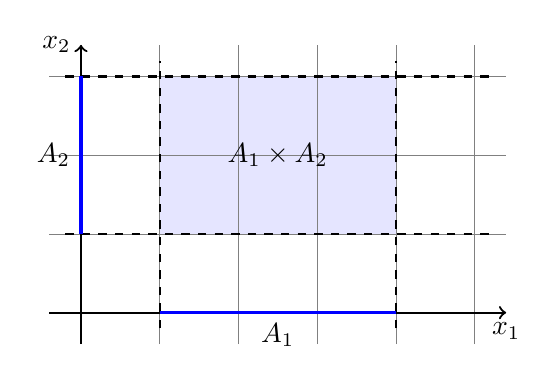
\begin{tikzpicture}
            \fill[blue!10!white] (1,1) rectangle (4,3);
            \draw[step=1cm,gray,very thin] (-0.4,-0.4) grid (5.4,3.4);
            \draw[thick,->] (-0.4,0) -- (5.4,0) node[anchor=north]{\(x_1\)};
            \draw[thick,->] (0,-0.4) -- (0,3.4) node[anchor=east]{\(x_2\)};
            \draw[thick,dashed] (1,-0.2) -- (1,3.2);
            \draw[thick,dashed] (4,-0.2) -- (4,3.2);
            \draw[thick,dashed] (-0.2,1) -- (5.2,1);
            \draw[thick,dashed] (-0.2,3) -- (5.2,3);
            \draw[blue, very thick] (1,0) -- (4,0) node[black,midway,below]{\(A_1\)};
            \draw[blue, very thick] (0,1) -- (0,3) node[black,midway,left]{\(A_2\)};
            \node[] at (2.5,2) {\(A_1 \times A_2\)};
        \end{tikzpicture}
        \caption{If \(A_1, A_2\) are intervals then \( A_1 \times A_2 \) is a rectangle.}
    \end{centering}
\end{figure}

Discussing the ``interior'' of the set naturally suggests the topic of the ``boundary'' of the set.
In the following definitions we develop this idea.


\begin{definition}[exterior points]
    Let \(S\subset \bR^n\).
    A point \(\aa \notin S\) is said to be an \emph{exterior point} if there exists \(r>0\) such that \(B(\aa,r)\cap S = \emptyset\).
    The set of all exterior points of \(S\) is denoted \(\operatorname{ext} S\).
\end{definition}

Observe that \(\operatorname{ext} S\) is an open set.
We use the notation \(S^c = \bR^n \setminus S\) and we say that \(C^c\) is the \emph{complement} of the set \(S\).



\begin{definition}[boundary]
    The set \(\bR^n \setminus (\operatorname{int} S \cup \operatorname{ext} S )\) is called the boundary of \(S \subset \bR^n\) and is denoted \(\partial S\).
\end{definition}


\begin{definition}[closed]
    A set \(S\subset \bR^n\) is said to be \emph{closed} if \(\partial S \subset S\).
\end{definition}

\begin{lemma}
    \(S\) is open \(\Longleftrightarrow \) \(S^c\) is closed.
\end{lemma}
\begin{proof}
    Observe that \(\bR^n =  \operatorname{int} S \cup \partial S \cup \operatorname{ext} S\) (disjointly).
    If \(\xx \in \partial S\) then, for every \(r>0\), \(B(\xx,r) \cap S \neq \emptyset\) and so \(\xx \in \partial(S^c)\).
    Similarly with \(S\) and \(S^c\) swapped and so \(\partial S = \partial(S^c)\).
    If \(S\) is open then \(\operatorname{int} S = S\) and \(S^c = \operatorname{ext} S \cup \partial S =  \operatorname{ext} S \cup \partial (S^c)\) and so \(S^c\) is closed.
    If \(S\) is not open then there exists \(\aa \in \partial S \cap S\). Additionally  \(\aa \in \partial (S^c) \cap S\) hence \(S^c\) is not closed.
\end{proof}


\subsection*{Limits and continuity}

Let \(S\subset \bR^n\) and \(\ff : S \to \bR^m\).
If \(\aa\in \bR^n\), \(\bb\in \bR^m\) we write
    {\(  \displaystyle\lim_{\xx \to \aa}\ff(\xx) = \bb \)}
to mean that
\(\lim_{\norm{\xx-\aa}\to 0}\norm{\ff(\xx)-\bb}=0\).
Observe how, if \(n=m=1\), this is the familiar notion of continuity for functions on \(\bR\).

\begin{definition}[continuous]
    A function \(\ff\) is said to be \emph{continuous} at \(\aa\) if \(\ff\) is defined at \(\aa\) and
    \(  \displaystyle\lim_{\xx \to \aa}\ff(\xx) = \ff(\aa)\).
    We say \(\ff\) is continuous on \(S\) if \(\ff\) is continuous at each point of \(S\).
\end{definition}

\begin{theorem}
    Suppose that \(  \lim_{\xx \to \aa}\ff(\xx) = \bb\) and \(  \lim_{\xx \to \aa}\gg(\xx) = \cc\).
    Then
    \begin{enumerate}
        \item \(  \lim_{\xx \to \aa}(\ff(\xx)+\gg(\xx)) = \bb+\cc\),
        \item \(  \lim_{\xx \to \aa} \lambda \ff(\xx) = \lambda \bb\) for every \(\lambda \in \bR\),
        \item \(  \lim_{\xx \to \aa}\ff(\xx)\cdot \gg(\xx) = \bb\cdot \cc\),
        \item \(  \lim_{\xx \to \aa} \norm{\ff(\xx)} = \norm{\bb}\).
    \end{enumerate}
\end{theorem}

We prove a couple of the parts of the above theorem here, the other parts are left as exercises and are relatively straightforward.

\begin{proof}[Proof of (c)]
    Observe that  \(
    \ff(\xx)\cdot\gg(\xx) - \bb\cdot \cc
    = (\ff(\xx)-\bb)\cdot(\gg(\xx)-\cc) + \bb\cdot(\gg(\xx)-\cc) + \cc\cdot(\ff(\xx)-\bb)
    \).
    By the triangle inequality and Cauchy-Schwarz,
    \[
        \begin{aligned}
            \norm{\ff(\xx)\cdot\gg(\xx) - \bb\cdot \cc }
             & \leq \norm{\ff(\xx)-\bb} \norm{\gg(\xx)-\cc} \\
             & \quad + \norm{\bb}\norm{\gg(\xx)-\cc}        \\
             & \quad + \norm{\cc} \norm{\ff(\xx)-\bb}.
        \end{aligned}
    \]
    Since \(\norm{\ff(\xx)-\bb} \to 0\) and \(\norm{\gg(\xx)-\cc} \to 0\) as \(\xx \to \aa\) this implies that \(\norm{\ff(\xx)\cdot\gg(\xx) - \bb\cdot \cc }\to 0\).
\end{proof}

\begin{proof}[Proof of (d)]
    Take \(\ff = \gg\) in part (c) implies that \(   \lim_{\xx \to \aa} \norm{\ff(\xx)}^2 = \norm{\bb}^2\).
\end{proof}


When writing a vector field (or similar functions) it is often convenient to divided the higher-dimensional function into smaller parts.
We call these parts the \emph{components of a vector field}.

\begin{theorem}
    Let \(\ff(\xx) = \left(f_1(\xx),\ldots,f_m(\xx) \right)\).
    Then \(\ff\) is continuous if and only if each \(f_k\) is continuous.
\end{theorem}
\begin{proof}
    \begin{description}
        \item[(\(\Rightarrow\))]
            Let
            \( \ee_k=(0,\ldots,0,\here{1}{fromHere},0,\ldots,0)  \)
            \begin{tikzpicture}[remember picture, overlay]
                \node[font=\scriptsize, above right=7pt of fromHere] (toHere) {$k$\textsuperscript{th}position};
                \draw[<-] ([yshift=4pt]fromHere.north) |- (toHere);
            \end{tikzpicture}
            and observe that \(f_k(\xx) = \ff(\xx)\cdot \ee_k\).
            We have already shown that the continuity of two vector fields implies the continuity of the inner product.
        \item[(\(\Leftarrow \))]
            By definition of the norm
            \(\norm{\ff(\xx)-\ff(\aa)}^2 = \displaystyle\sum_{k=1}^{m}(f_k(\xx)-f_k(\aa))^2\)
            and we know \(\norm{f_k(\xx)-f_k(\aa)} \to 0\) as \(\norm{\xx-\aa}\to 0\). \qedhere
    \end{description}
\end{proof}



\begin{example*}[polynomials]
    A  \emph{polynomial} in \(n\) variables is a scalar field on \(\bR^n\) of the from
    \[
        p(x_1,\ldots,x_n)
        = \sum_{k_1=0}^{j}\cdots \sum_{k_n=0}^{j} c_{k_1,\dots,k_n} x_1^{k_1}\cdots x_n^{k_n}.
    \]
    E.g., \(f(x_1,x_2):= x_1 + 2x_1x_2 - x_1^2\) is a polynomial in \(2\) variables.
    Polynomials are continuous everywhere in \(\bR^n\). (Finite sum of products of continuous fields.)
\end{example*}

\begin{example*}[rational functions]
    A  \emph{rational function} is a scalar field
    \[
        f(\xx)=\frac{p(\xx)}{q(\xx)}
    \]
    where \(p(\xx)\) and \(q(\xx)\) are polynomials.
    A rational function is continuous at every point \(\xx\) such that \(q(\xx)\neq 0\).
\end{example*}

The continuity of functions continues to hold, in an intuitive way, under composition of functions.

\begin{theorem}
    Suppose \(S \subset \bR^l\), \(T\subset \bR^m\), \(\ff:S \to \bR^m\), \(\gg : T \to \bR^n\) and that \(\ff(S) \subset T\) so that
    \[(\gg \circ \ff)(\xx) = \gg(\ff(\xx))\]
    makes sense.
    If \(\ff\) is continuous at \(\aa\in S\) and \(\gg\) is continuous at \(\ff(\aa)\) then \(\gg\circ \ff\) is continuous at \(\aa\).
\end{theorem}

\begin{proof}
    \(\displaystyle\lim_{\xx\to\aa}\norm{\ff(\gg(\xx))-\ff(\gg(\aa))}  =\displaystyle\lim_{\yy\to\gg(\aa)}\norm{\ff(\yy)-\ff(\gg(\aa))}  =0   \)
\end{proof}

\begin{example*}
    We can consider the scalar field \(f(x,y)= \sin(x^2 + y) + x y\) as the composition of functions.
\end{example*}



\begin{example*}[continuity in higher dimensions]
    Let \(f(x,y)\) be defined as \(f(0,0)=0\) and, for all \((x,y)\neq (0,0)\),
    \[
        f(x,y) =
        \frac{x y}{x^2 + y^2}.
    \]
    What is the behaviour of \(f\) when approaching \((0,0)\) along the following three lines?
    \begin{center}
        \begin{tabular}{ c | c }
            line         & value                     \\
            \hline
            \(\{x=0\}\)  & \(f(0,t) =  0\)           \\
            \(\{y=0\}\)  & \(f(t,0) = 0\)            \\
            \(\{x=y\}\)  & \(f(t,t) = \frac{1}{2}\)  \\
            \(\{x=-y\}\) & \(f(t,t) =-\frac{1}{2}\).
        \end{tabular}
    \end{center}
\end{example*}



\section{Derivatives of scalar fields}


\begin{figure}
    \begin{center}
        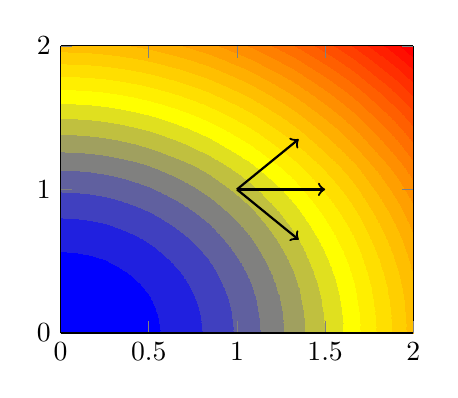
\begin{tikzpicture}
            \begin{axis}[
                    view={0}{90},
                    width = .5\textwidth]
                \addplot3[
                    domain=0:2,
                    domain y=0:2,
                    contour filled={number=25}]
                {x*x + y*y};
                \draw[->,thick] (axis cs:1,1) -- (axis cs:1.35,1.35); %\node[midway, left]{\(\left(\begin{smallmatrix}0 \\ 1\end{smallmatrix} \right)\)};
                \draw[->,thick] (axis cs:1,1) -- (axis cs:1.5,1);
                \draw[->,thick] (axis cs:1,1) -- (axis cs:1.35,0.65);
            \end{axis}
        \end{tikzpicture}
        \caption{Plot where colour represents the value of \(f(x,y)=x^2 + y^2\). The change in \(f\) depends on direction.}
    \end{center}
\end{figure}




\begin{definition}[directional derivative]
    Let \(S\subset \bR^n\) and \(f:S\to \bR\).
    For any \(\aa \in \operatorname{int}S\) and \(\vv \in \bR^n\), \(\norm{v}=1\) the derivative of \(f\) with respect to \(\vv\) is defined as
    \[
        D_{\vv}f(\aa) :=
        \lim_{h\to 0} \frac{1}{h}\left(  f(\aa+h \vv) - f(\aa)     \right).
    \]
\end{definition}


When \(h\) is small we can guarantee that \(\aa + h \vv \in S\) because \(\aa\in \operatorname{int} S\) so this definition makes sense.




\begin{theorem}
    Suppose \(S\subset \bR^n\), \(f:S\to \bR\), \(\aa \in \operatorname{int} S\).
    Let \(g(t) := f(\aa + t\vv)\).
    If one of the derivatives \(g'(t)\) or \(D_\vv f(\aa)\) exists then the other also exists and
    \[
        g'(t) = D_{\vv}f(\aa+t \vv).
    \]
    In particular \(g'(0) = D_{\vv}f(\aa)\).
\end{theorem}

%<>{Note:}

\begin{proof}
    By definition \(\frac{1}{h}(g(t+h)-g(h)) =\frac{1}{h}(f(\aa+h \vv) - f(\aa)) \).
\end{proof}

\begin{theorem*}[mean value]
    Assume that \(D_{\vv}(\aa+t\vv)\)  exists for each \(t\in [0,1]\). Then for some \(\theta \in (0,1)\),
    \[
        f(\aa+\vv) - f(\aa) = D_{\vv}f (\zz),
        \quad
        \text{where \(z=\aa + \theta \vv\)}.
    \]
\end{theorem*}

\begin{proof}
    Apply mean value theorem to \(g(t) = f(\aa+t\vv)\).
\end{proof}





% \tikzset{external/export next=false}
For any \(k\in\{1,2,\ldots,n\}\),
let
\( \ee_k=(0,\ldots,0,\here{\(1\)}{fromHere},0,\ldots,0)  \).
\begin{tikzpicture}[remember picture, overlay]
    \node[font=\scriptsize, above right=7pt of fromHere] (toHere) {$k$\textsuperscript{th}position};
    \draw[<-] ([yshift=4pt]fromHere.north) |- (toHere);
\end{tikzpicture}

\begin{definition}[partial derivatives]
    We define the \emph{partial derivative} in \(x_k\) of \(f(x_1,x_2,\ldots,x_n)\) at \(\aa\) as
    \[
        \frac{\partial f}{\partial x_k}(\aa) := D_{\ee_k}f(\aa).
    \]
\end{definition}



Various symbols used for partial derivatives:
\(\frac{\partial f}{\partial x_k}(\aa) = D_kf(\aa) = \partial_{k}f(\aa)\).
If  a function is written \(f(x,y)\) we write \(\frac{\partial f}{\partial x}, \frac{\partial f}{\partial y}\) for the partial derivatives. Similarly for higher dimension.
In practice, to compute the partial derivative \( \frac{\partial f}{\partial x_k}\), one should consider all other \(x_j\) for \(j\neq k\) as constants and take the derivative with respect to \(x_k\).


If \(f:\bR \to \bR\) is differentiable, then
\[
    f(a + h) = f(a) + h f'(a) + hE(a,h)
\]
where \(E(a,h) \to 0\) as \(h\to 0\).
I.e., \(f(a) + hf'(a)\) approximates \(f(x)\) close to \(a\).


\begin{definition}[differentiable]
    Let \(S\subset \bR^n\) be open, \(f:S \to \bR\).
    We say that \(f\) is \emph{differentiable} at \(\aa \in S\) if there is \(T_\aa \in \bR^n\) and \(E(\aa,\vv)\) such that, for \(\vv\in B(\aa,r)\),
    \[
        f(\aa+\vv) = f(\aa) + T_\aa \cdot \vv + \norm{\vv}E(\aa,\vv)
    \]
    and \(E(\aa,\vv) \to 0\) as \(\vv \to 0\).
\end{definition}

\begin{theorem}
    If \(f\) is differentiable at \(\aa\)
    then \(T_\aa = \left( \partial_1 f(\aa), \ldots, \partial_nf(\aa) \right)\)
    and \(D_{\vv}f(\aa) = T_{\aa}\cdot \vv\).
\end{theorem}



\begin{proof}
    Since \(f\) is differentiable
    \(  f(\aa+ h \vv) = f(\aa) + h T_\aa \cdot \vv + h\norm{\vv}E(\aa,h\vv)\)
    and hence
    \[
        D_{\vv}f(\aa) :=
        \lim_{h\to 0} \frac{f(\aa+h \vv) - f(\aa)}{h}
        =
        \lim_{h\to 0} \frac{ h T_\aa \cdot \vv + h\norm{\vv}E(\aa,h\vv) }{h}
        = T_\aa \cdot \vv.
    \]
    In particular \(T_\aa\cdot \ee_k = D_{\ee_k}f(\aa)\).
\end{proof}





%
\begin{definition}[gradient]
    The \emph{gradient} of \(f\) is the vector-valued function
    \[
        \nabla f(\aa) :=
        \begin{pmatrix}
            \partial_1 f(\aa) \\
            \partial_2 f(\aa) \\
            \vdots            \\
            \partial_nf(\aa)
        \end{pmatrix}.
    \]
\end{definition}
%




\begin{theorem*}
    If \(f\) is differentiable at \(\aa\), then it is continuous at \(\aa\).
\end{theorem*}
\begin{proof}
    \begin{align*}
         & \abs{f(\aa+\vv)-f(\aa)}                                                            \\
         & \quad = \abs{ T_\aa \cdot \vv + \norm{\vv}E(\aa,\vv)  }                            \\
         & \quad \leq  \norm{T_\aa } \norm{\vv} + \norm{\vv} \abs{E(\aa,\vv)} \to 0. \qedhere
    \end{align*}
\end{proof}







{}

\begin{theorem}
    Suppose that the partial derivatives \(\partial_1 f(\xx), \partial_2 f(\xx), \ldots, \partial_nf(\xx)\) exist for all \(\xx\in B(\aa,r)\) and are continuous at \(\aa\).
    Then \(f\) is differentiable at \(\aa\).
\end{theorem}
\begin{proof}

    \begin{enumerate}
        \item Write \(\vv = (v_1,v_2,\ldots,v_n)\)
              and
              \(\uu_k = (v_1,v_2,\ldots,v_k,0,\ldots,0)\);
        \item Observe that \(\uu_k - \uu_{k-1} = v_k \ee_k\), \(\uu_0 = (0,0,\ldots,0)\) and \(\uu_n = \vv\);
        \item Using the mean value theorem (exists \( \zz_k = \uu_{k-1}+ \theta_k \ee_k\)) \vspace{-0.9em}
              \[
                  \begin{aligned}
                      f(\aa+\vv) - f(\aa)
                       & = \sum_{k=1}^{n} f(\aa + \uu_k) - f(\aa + \uu_{k-1})
                      = \sum_{k=1}^{n} v_k  D_{\ee_k}f(\aa +  \zz_k)                                                                  \\
                       & = \sum_{k=1}^{n} v_k  D_{\ee_k}f(\aa + \uu_{k-1})                                                            \\
                       & \ \ \ \ \ \ \ \ + \sum_{k=1}^{n}  v_k \left(  D_{\ee_k}f(\aa +  \zz_k)-  D_{\ee_k}f(\aa + \uu_{k-1}) \right)
                  \end{aligned}
              \]
        \item \(\sum_{k=1}^{n} v_k  D_{\ee_k}f(\aa + \uu_{k-1}) \to \vv \cdot \nabla f(\aa)\). \qedhere
    \end{enumerate}
\end{proof}




% 
%     {Parametrized curves}

%     Let \(\rr(t) = \left( X_1(t), \ldots, X_n(t)  \right)\) be a vector-valued function defined on an interval \(I\subset \bR\).
%     This describes a curve in \(\bR^n\).


%     \begin{example*}
%         \begin{itemize}
%             \item         \(\rr(t) = (\cos t, 2 \sin t)\), \(t\in [0,2\pi]\)
%             \item  \(\rr(t) = (\cos t, \sin t, t)\), \(t\in \bR\)
%         \end{itemize}

%     \end{example*}

%     Different ways of describing a curve.
% 

\subsection*{Chain rule}

If \(f(t) = g\circ h(t)\) then \(f'(t) = g'(h(t)) \ h'(t)\).
Does this extend to higher dimension?

\begin{example*}
    Suppose that
    \begin{itemize}
        \item \(\xx:\bR \to \bR^3\) describes the position \(\xx(t)\) at time \(t\),
        \item \(f:\bR^3 \to \bR\) describes the temperature \(f(\xx)\) at a point \(\xx\)
    \end{itemize}

    The temperature at time \(t\) is equal to \(g(t)=f(\xx(t))\).
    We want to calculate \(g'(t)\).
\end{example*}






{Derivative of \(\aalpha:\bR \to \bR^n\)}


Let \(\aalpha:\bR \to \bR^n\) and suppose it has the form
\(\aalpha(t) = \left( \alpha_1(t), \ldots, \alpha_n(t)  \right)\).
We define the derivative as
\[
    \aalpha'(t) := \begin{pmatrix}
        x_1'(t) \\
        \vdots  \\
        x_n'(t)
    \end{pmatrix}.  % = \left( x_1'(t), \ldots, x_n'(t)  \right).
\]

Here \(\aalpha'\) is a vector-valued function which represents the ``direction of movement''.

% We sometimes consider horizontal and sometimes vertical vectors. It can be convenient to distinguish between ``position'' and ``direction''.


\begin{figure}[htb]
    \begin{center}
        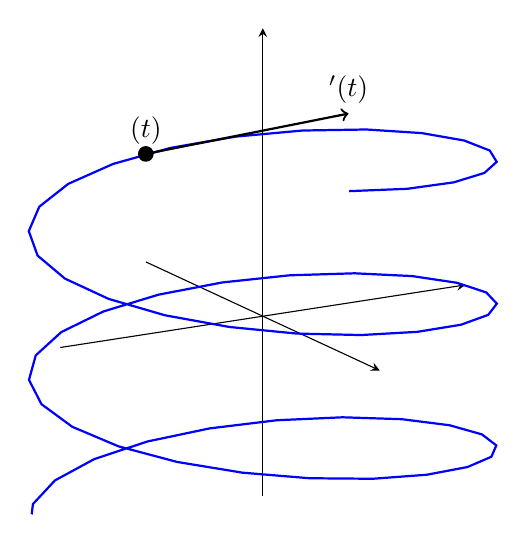
\begin{tikzpicture}%
            \begin{axis}[
                    view={60}{15},
                    width=0.8\textwidth,
                    height=0.8\textwidth,
                    axis lines=center,
                    xlabel=$ $,ylabel=$ $,zlabel=$ $,
                    zmin=-1, zmax=1.6,
                    xtick=\empty,  ytick=\empty,  ztick=\empty
                ]
                \addplot3[blue,thick,domain=-9:8,samples=60,samples y=0]
                ({sin(deg(x))},
                {cos(deg(x))},
                {2*x/(5*pi)});
                \draw[->,thick] (axis cs:-1,0,0.6) -- (axis cs:-1,1,0.65) node[anchor=south]{\(\aalpha'(t)\)};
                \node[circle,fill,inner sep=2pt] at (axis cs:-1,0,0.6) {} ;
                \node[anchor=south] at (axis cs:-1,0,0.6) {\(\aalpha(t)\)} ;
            \end{axis}
        \end{tikzpicture}
        \caption{\(\aalpha(t)=(\cos t, \sin t, t)\), \(t\in \bR\).}
    \end{center}
\end{figure}


\begin{theorem*}
    Let \(S\subset \bR^n\) be open and \(I\subset \bR\) an interval.
    Let \(\xx: I \to S\) and \(f:S \to \bR\) and define, for \(t\in I\),
    \[
        g(t) = f (\xx(t)).
    \]
    Suppose that  \(t\in I\) is such that \(\xx'(t)\) exists and \(f\) is differentiable at \(\xx(t)\).
    Then \(g'(t)\) exists and
    \[
        g'(t) = \nabla f \left(\xx(t)\right) \cdot \xx'(t).
    \]
\end{theorem*}


\begin{proof}
    Let \(h>0\) be small, \vspace{-.5em}
    \[
        \begin{aligned}
            \tfrac{1}{h}\left[g(t+h)-g(t) \right]
             & = \tfrac{1}{h}\left[f(\xx(t+h)-f(\xx(t)))\right]                        \\
             & = \tfrac{1}{h} \nabla f(\xx(t))\cdot (\xx(t+h)-\xx(t))                  \\
             & \ \ +  \tfrac{1}{h}  \norm{\xx(t+h)-\xx(t)} E(\xx(t), \xx(t+h)-\xx(t)).
        \end{aligned}
    \]
    Observe that \(\tfrac{1}{h}  (\xx(t+h)-\xx(t)) \to \xx'(t)  \) as \(h\to 0\).
\end{proof}


\begin{example*}
    A particle moves in a circle and its position at time \(t\in [0,2\pi]\) is given by
    \[
        \xx(t) = (\cos t, \sin t).
    \]
    The temperature at a point \(\yy=(y_1,y_2)\) is given by the function \(f(\yy) := y_1 + y_2\),
    The temperature the particle experiences at time \(t\) is given by \(g(t) = f (\xx(t))\).
    Temperature change:
    \(
    g'(t)
    = \nabla f \left(\xx(t)\right) \cdot \xx'(t)
    = \left(\begin{smallmatrix}
            1 \\
            1
        \end{smallmatrix}\right)
    \cdot
    \left( \begin{smallmatrix}
            -\sin t \\
            \cos t
        \end{smallmatrix}\right)
    = \cos t - \sin t.
    \)
\end{example*}


\begin{figure}
    \begin{center}
        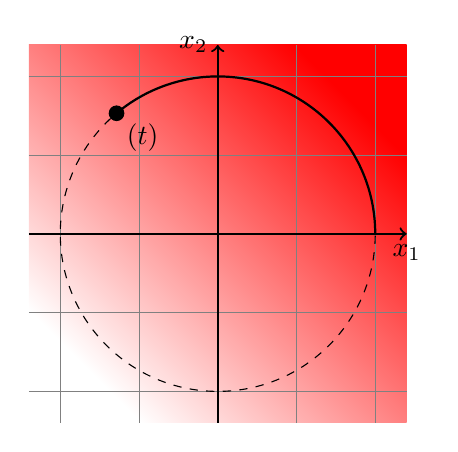
\begin{tikzpicture}
            \shade[shading=axis, top color=red, shading angle=-45] (-2.4,-2.4) rectangle (2.4,2.4);
            \draw[step=1cm,gray,very thin] (-2.4,-2.4) grid (2.4,2.4);
            \draw[thick,->] (-2.4,0) -- (2.4,0) node[anchor=north]{\(x_1\)};
            \draw[thick,->] (0,-2.4) -- (0,2.4) node[anchor=east]{\(x_2\)};
            \draw[dashed] (0,0) circle (2);
            \draw[thick] (2,0) arc [start angle=0, end angle=130, radius=2] node[circle,fill,inner sep=2pt]{} node[anchor=north west]{\(\xx(t)\)};
        \end{tikzpicture}
        \caption{\(\xx(t)\) is the position of a particle. Shading represents temperature \(f\).}
    \end{center}
\end{figure}






\section{Level sets \& tangent planes}

Let \(S\subset \bR^2\), \(f:S\to\bR\).
Suppose \(c\in \bR\) and
\[
    L(c) := \left\{\xx\in S : f(\xx)=c\right\}
\]
is a curve at \(\aa \in S\) in the sense that  \(\xx:I \to S\) is the parametric form of the curve.
The set \(L(c)\) is called the \emph{level set}.
I.e., \(\xx(t_a) = \aa\) for some \(t_a \in I\) and \[f(\xx(t))=c\] for all \(t\in I\).
Then
\begin{itemize}
    \item \(\nabla f(\aa)\) is normal to the curve at \(\aa\)
    \item Tangent line at \(\aa\) is
          \(\left\{\xx\in\bR^2: \nabla f(\aa) \cdot (\xx-\aa)=0\right\}\)
\end{itemize}

This is because the chain rule implies that \(\nabla f(\xx(t)) \cdot \xx'(t) = 0\).

% \begin{figure}
%     \begin{tikzpicture}
%         \begin{axis}[
%                 view={0}{90},
%                 small,
%             ]
%             \addplot3[
%                 domain=-1.3:1.3,
%                 domain y=-1.3:1.3,
%                 contour gnuplot={number=14},
%                 thick,
%             ]
%             {exp(-x^2-y^2)*x};
%         \end{axis}
%     \end{tikzpicture}
%     \caption{Contour plot of \(x_1 \exp(-x_1^2-x_2^2)\)}
% \end{figure}

\begin{itemize}
    \item   Isotherms \(\leftrightarrow\) temperature;
    \item   Contours \(\leftrightarrow\)  altitude.
\end{itemize}

\begin{example*}
    Let \(f(x_1,x_2,x_3):=x_1^2 + x_2^2 + x_3^2\).
    \begin{itemize}
        \item If \(c>0\) then \(L(c)\) %\(L(c) = \left\{(x_1,x_2,x_3):  x_1^2 + x_2^2 + x_3^2 = c\right\}\)
              is a sphere,
        \item \(L(0) \) is a single point \((0,0,0)\),
        \item If \(c<0\) then \(L(c)\) is empty.
    \end{itemize}
\end{example*}

\begin{example*}
    Let \(f(x_1,x_2,x_3):=x_1^2 + x_2^2 - x_3^2\).
    \begin{itemize}
        \item If \(c>0\) then \(L(c)\) is a one-sheeted hyperboloid,
        \item \(L(0) \) is an infinite cone,
        \item If \(c<0\) then \(L(c)\) is a two-sheeted hyperboloid.
    \end{itemize}
\end{example*}

%
% %                       
\begin{figure}
    \begin{center}
        \begin{minipage}[c]{0.5\textwidth}
            %\fbox{
            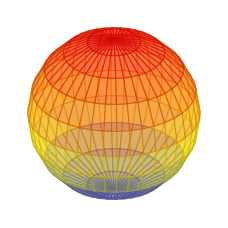
\begin{tikzpicture}
                \begin{axis}[hide axis,axis equal]
                    \addplot3[%
                        opacity = 0.5,
                        surf,
                        z buffer = sort,
                        samples = 21,
                        variable = \u,
                        variable y = \v,
                        domain = 0:180,
                        y domain = 0:360,
                    ]
                    ({cos(u)*sin(v)}, {sin(u)*sin(v)}, {cos(v)});
                \end{axis}
            \end{tikzpicture}%
            %}
        \end{minipage}%
        \begin{minipage}[c]{0.5\textwidth}
            %\fbox{
            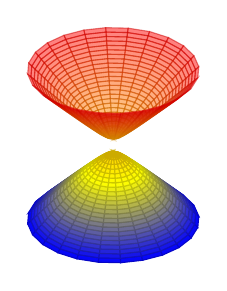
\begin{tikzpicture}
                \begin{axis}[hide axis,axis equal]
                    \addplot3[surf, opacity = 0.5,                     z buffer = sort, domain=0:360,y domain=.2:2]
                    ({sqrt(y*y-.04)*cos(x)},{sqrt(y*y-.04)*sin(x)},{y});
                    \addplot3[surf,domain=0:360,y domain=-2:-.2]
                    ({sqrt(y*y-.04)*cos(x)},{sqrt(y*y-.04)*sin(x)},{y});
                \end{axis}
            \end{tikzpicture}
            %}
        \end{minipage}%

        \begin{minipage}[c]{0.5\textwidth}
            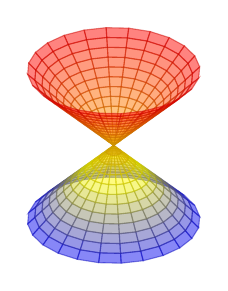
\begin{tikzpicture}
                \begin{axis}[hide axis,axis equal]
                    \addplot3[surf, opacity = 0.5,domain=0:360,y domain=-2:2]
                    ({y*cos(x)},{y*sin(x)},{y});
                \end{axis}
            \end{tikzpicture}%                
        \end{minipage}%
        \begin{minipage}[c]{0.5\textwidth}
            %\fbox{
            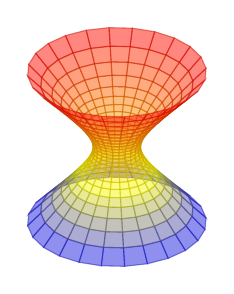
\begin{tikzpicture}
                \begin{axis}[hide axis,axis equal]
                    \addplot3[surf, opacity = 0.5,domain=0:360,y domain=-2:2]
                    ({cosh(y)*cos(x)},{cosh(y)*sin(x)},{sinh(y)});
                \end{axis}
            \end{tikzpicture}
            %}
        \end{minipage}
        \caption{Sphere, two-sheeted hyperboloid, infinite cone, one-sheeted hyperboloid.}
    \end{center}
\end{figure}


Let \(f\) be a differentiable scalar field on \(S\subset \bR^3\) and suppose that \(L(c) = \left\{\xx\in S : f(\xx)=c\right\}\) is a surface.

\begin{itemize}
    \item \(\nabla f(\aa)\) is normal to every curve \(\aalpha(t)\) in the surface which passes through \(\aa\),
    \item Tangent plane at \(\aa\) is
          \(\left\{\xx\in\bR^3: \nabla f(\aa) \cdot (\xx-\aa)=0\right\}\).
\end{itemize}

Same argument as in \(\bR^2\) works in \(\bR^n\).




% \begin{figure}
%     \noindent\begin{tikzpicture}%
%         \node[anchor=south west,inner sep=0] (image) at (0,0)
%         {\includesvg[width=\textwidth,inkscapelatex=false]{tangent}};
%         % SVG adapted from work in public domain (https://commons.wikimedia.org/wiki/File:Tangentialvektor.svg)
%         \begin{scope}[x={(image.south east)},y={(image.north west)}]
%             % scope for unitary coordinates over image
%             \node[] at (0.5,1) {\(\nabla f(\aa)\)};
%             \node[] at (0.43,0.75) {\(\aa\)};
%             \node[] at (0.8,0.48) {\(L(c)\)};
%             \node[] at (0.1,0.27) {\(\aalpha(t)\)};
%             \node[] at (0.17,0.75) {\(\aalpha'(t)\)};
%         \end{scope}
%     \end{tikzpicture}
%     \caption{Tangent plane and normal vector}
% \end{figure}





\section{Derivatives of vector fields}



 {Derivatives of vector fields}

\begin{definition}[Directional derivative]
    Let \(S\subset \bR^n\) and \(\ff:S\to \bR^m\).
    For any \(\aa \in \operatorname{int}S\) and \(\vv \in \bR^n\) the derivative of \(f\) with respect to \(\vv\) is defined as
    \[
        D_{\vv}\ff(\aa) :=
        \lim_{h\to 0} \frac{\ff(\aa+h \vv) - \ff(\aa)}{h}.
    \]
\end{definition}

Note: If we write \(\ff = (f_1,\ldots,f_m)\) then \(D_{\vv}\ff = (D_{\vv}f_1,\ldots,D_{\vv} f_m)\).


\begin{definition}[Differentiable]
    We say that \(f\) is \emph{differentiable} at \(\aa\) if there is a linear transformation \(\mathbf{T}_\aa : \bR^n \to \bR^m\) and \(\mathbf{E}(\aa,\vv)\) such that, for \(\vv\in B(\aa,r)\),
    \[
        \ff(\aa+\vv) = \ff(\aa) + \mathbf{T}_\aa  (\vv )+ \norm{\vv}\mathbf{E}(\aa,\vv)
    \]
    and \(\mathbf{E}(\aa,\vv) \to 0\) as \(\vv \to 0\).
\end{definition}


\begin{theorem}
    If \(\ff\) is differentiable at \(\aa\)
    then \(\ff\) is continuous at \(\aa\)
    and \( \mathbf{T}_{\aa}( \vv) =D_{\vv}\ff(\aa) \).
\end{theorem}

\begin{proof}
    Same as for the case when \(f:\bR^n \to \bR\).
\end{proof}


\section{Jacobian matrix and chain rule}


\begin{definition}[Jacobian matrix]
    The \emph{Jacobian matrix} of \(\ff : \bR^n \to \bR^m\) at \(\aa\) is defined as
    \[
        D\ff(\aa) =
        \begin{pmatrix}
            \partial_1 f_1 (\aa) & \partial_2 f_1 (\aa) & \cdots & \partial_n f_1 (\aa) \\
            \partial_1 f_2 (\aa) & \partial_2 f_2 (\aa) & \cdots & \partial_n f_2 (\aa) \\
            \vdots               & \vdots               &        & \vdots               \\
            \partial_1 f_m (\aa) & \partial_2 f_m (\aa) & \cdots & \partial_n f_m (\aa)
        \end{pmatrix}
    \]

\end{definition}




\begin{itemize}
    \item Choosing a basis any linear transformation can be written as a \(m \times n\) matrix.
    \item \( \mathbf{T}_\aa  (\vv ) = D\ff(\aa) \vv\).
\end{itemize}



{Derivatives of \(\ff : \bR^n \to \bR^m\) (recap.)}


Let \(S\subset \bR^n\) and \(\ff : S \to \bR^m\).
If \(f\) is differentiable at \(\aa \in S\) then, for all  \(\vv\in B(\aa,r) \subset S\),
\[
    \ff(\aa+\vv) = \ff(\aa) +  D\ff(\aa) \vv + \norm{\vv}\mathbf{E}(\aa,\vv).
\]


This is like a Taylor expansion in higher dimensions.


Here we see that in higher dimensions we have a matrix form of the chain rule.

\begin{theorem}
    Let \(S\subset \bR^l\), \(T\subset \bR^m\) be open.
    Let \(\ff: S \to T\) and \(\gg:T \to \bR^n\) and define
    \[
        \hh := \gg \circ \ff : S \to \bR^n.
    \]
    Let  \(\aa\in S\). Suppose that \(\ff\) is differentiable at \(\aa\) and \(\gg\) is differentiable at \(\ff(\aa)\).
    Then \(\hh\) is differentiable at \(\aa\) and
    \[
        D\hh(\aa) = D\gg(\ff(\aa)) \ D\ff(\aa).
    \]
\end{theorem}

\vspace{-1em}

\begin{proof}
    Since \(\ff\) and \(\gg\) are differentiable there exists \(\mathbf{E}_{\ff}\) and \(\mathbf{E}_{\gg}\).
    Let \(\uu := \ff(\aa+\vv) - \ff(\aa) \).
    \[
        \begin{aligned}
            \hh(\aa+\vv) - \hh(\aa)
             & = \gg(\ff(\aa+\vv)) - \ff(\hh(\aa))                                                                                               \\
             & = D\gg(\ff(\aa))(\ff(\aa+\vv) - \ff(\aa) ) + \norm{\uu}\mathbf{E}_{\gg}(\ff(\aa),\uu)                                             \\
             & = D\gg(\ff(\aa))   D\ff(\aa) \vv + \norm{\vv}D\gg(\ff(\aa))\mathbf{E}_{\ff}(\aa, \vv) + \norm{\uu}\mathbf{E}_{\gg}(\ff(\aa),\uu).
        \end{aligned} \qedhere
    \]
\end{proof}




{Polar coordinates (derivatives example)}


\begin{itemize}
    \item
          We can write the change of coordinates
          \((r,\theta) \mapsto (r\cos \theta, r\sin \theta)\)
          as the function  \(\ff(r,\theta) = (x(r,\theta),y(r,\theta))\) where \(\ff:(0,\infty)\times [0,2\pi) \to \bR^2\).
    \item
          We calculate the Jacobian matrix
          \[
              D\ff(r,\theta) =
              \begin{pmatrix}
                  \partial_{r}x(r,\theta) & \partial_{\theta}x(r,\theta) \\
                  \partial_{r}y(r,\theta) & \partial_{\theta}y(r,\theta)
              \end{pmatrix}
              =
              \begin{pmatrix}
                  \cos \theta & -r\sin \theta \\
                  \sin \theta & r\cos \theta
              \end{pmatrix}.
          \]
    \item
          We wish to calculate derivatives of \(h := g \circ \ff\) for some  \(g:\bR^2 \to \bR\).
          \[
              \begin{aligned}
                  Dh(r,\theta) & = Dg(\ff(r,\theta)) \ D\ff(r,\theta) \\
                  \begin{pmatrix}
                      \partial_r h(r,\theta) & \partial_\theta h(r,\theta)
                  \end{pmatrix}
                               & =
                  \begin{pmatrix}
                      \partial_x g(\ff(r,\theta)) & \partial_y g(\ff(r,\theta))
                  \end{pmatrix}
                  \begin{pmatrix}
                      \cos \theta & -r\sin \theta \\
                      \sin \theta & r\cos \theta
                  \end{pmatrix}
              \end{aligned}
          \]

    \item Consequently
          \[
              \begin{cases}
                  \partial_r h(r,\theta) = \partial_x g(r\cos \theta, r\sin \theta) \cos \theta + \partial_y g(r\cos \theta, r\sin \theta)\sin \theta \\
                  \partial_\theta h(r,\theta) = - r \partial_x g(r\cos \theta, r\sin \theta) \sin \theta +  r \partial_y g(r\cos \theta, r\sin \theta)\cos \theta
              \end{cases}.
          \]
\end{itemize}






\section{Implicit functions and partial derivatives}


We consider the following equality of partial derivatives.
Imagining the application of the partial derivative we can convince ourselves that it is something reasonable.

Does \(\partial_1\partial_2 f = \partial_2\partial_1 f\), etc.?

\begin{example*}[partial derivative problem]
    Let \(f:\bR^2 \to \bR\) be defined as \(f(0,0)=0\) and, for \((x_1,x_2)\neq (0,0)\),
    \[
        f(x_1,x_2) := \frac{x_1x_2(x_1^2 - x_2^2)}{x_1^2 + x_2^2}.
    \]
    We can calculate \(\partial_2\partial_1 f (0,0) = -1\) but
    \(\partial_1\partial_2 f(0,0) = 1\).
\end{example*}

\begin{theorem}
    Let \(f:S\to\bR\) be a scalar field such that the partial derivatives \(\partial_1 f\), \(\partial_2 f\) and \(\partial_2\partial_1 f\) exist on an open set \(S\subset \bR^2\) containing \(\xx\).
    Further assume that \(\partial_2\partial_1 f\) is continuous on \(S\).
    Then the derivative \(\partial_1\partial_2 f(\xx)\) exists and \(\partial_1\partial_2 f(\xx)=\partial_2\partial_1 f(\xx)\).
\end{theorem}

% \begin{proof}
%     \dots Apostol Thm 8.8
% \end{proof}








Implicit
\begin{itemize}
    \item \(x^2-y=0\)
    \item \(x^2+y^2-1=0\)
    \item \(x^2-y^2-1=0\)
    \item \(x^2+y^2-e^y -4 =0\)
\end{itemize}

Explicit
\begin{itemize}
    \item \(f(x) = x^2\)
    \item \(f(x) = \pm \sqrt{1-x^2}\), \(\abs{x}\leq 1\)
    \item \(f(x) = \pm \sqrt{x^2-1}\), \(\abs{x}\geq 1\)
    \item ?
\end{itemize}





\begin{itemize}
    \item
          We know \(F:\bR^2 \to \bR\) and we suppose there exists some \(f:\bR\to\bR\) such that
          \(F(x,f(x))=0\) for all \(x\).
    \item
          Let \(g(x):= F(x,f(x))\) and note that \(g'(x)=0\).
    \item
          By the chain rule \(g'(x) \) is equal to
          \[
              \begin{pmatrix}
                  \partial_1 F(x,f(x)) & \partial_2 F(x,f(x))
              \end{pmatrix}
              \begin{pmatrix}
                  1 \\
                  f'(x)
              \end{pmatrix}
          \]
    \item
          Consequently
          \[
              f'(x) = - \frac{\partial_1 F(x,f(x))}{\partial_2 F(x,f(x))}.
          \]
    \item
          A similar argument holds in higher dimension.
\end{itemize}









